\documentclass[a4paper,12pt, ngerman,bibliography=totocnumbered ]{scrartcl}
\usepackage[a4paper]{geometry}


\geometry{a4paper,
        tmargin=3cm,
        bmargin=3cm,
        lmargin=3.6cm,
        rmargin=2.2cm,
        headheight=3em,
        headsep=2em,
        footskip=1cm}


\usepackage[onehalfspacing]{setspace}
\usepackage{epigraph}

\renewcommand{\familydefault}{\sfdefault}


\usepackage{amssymb}% http://ctan.org/pkg/amssymb
\usepackage{pifont}% http://ctan.org/pkg/pifont
\newcommand{\cmark}{\ding{51}}%
\newcommand{\xmark}{\ding{55}}%
\newcommand{\pmark}{\ding{48}}

\usepackage[utf8x]{inputenc}
\usepackage{graphicx}
\usepackage{float}

\usepackage{pdfpages}
\usepackage{wrapfig}

\PassOptionsToPackage{hyphens}{url}\usepackage[colorlinks,
pdfpagelabels,
urlcolor = black,
pdfstartview = FitH,
bookmarksopen = true,
bookmarksnumbered = true,
linkcolor = black,
plainpages = false,
hypertexnames = false,
citecolor = black,
breaklinks=true] {hyperref}




\usepackage[automark,headsepline]{scrlayer-scrpage}

\clearpairofpagestyles
\cfoot[\pagemark]{\pagemark}
\lehead{\headmark}
\rohead{\emph{\headmark}}
\setlength\parindent{0pt}

\definecolor{codeblack}{RGB}{83,83,83}
\definecolor{xdeepblack}{RGB}{64,64,64}

\renewcommand*{\headfont}{\color{xdeepblack}\bfseries}
\renewcommand*{\pnumfont}{\normalfont\bfseries}
\addtokomafont{paragraph}{\normalfont\color{xdeepblack}\bfseries}


\addtokomafont{descriptionlabel}{\color{xdeepblack}\normalfont\bfseries}

\definecolor{codegray}{rgb}{0.5,0.5,0.5}
\setheadsepline{1pt}[\color{codegray}]

%\urlstyle{tt}

\renewcommand{\UrlBreaks}{\do\/\do\a\do\b\do\c\do\d\do\e\do\f\do\g\do\h\do\i\do\j\do\k\do\l\do\m\do\n\do\o\do\p\do\q\do\r\do\s\do\t\do\u\do\v\do\w\do\x\do\y\do\z\do\A\do\B\do\C\do\D\do\E\do\F\do\G\do\H\do\I\do\J\do\K\do\L\do\M\do\N\do\O\do\P\do\Q\do\R\do\S\do\T\do\U\do\V\do\W\do\X\do\Y\do\Z}


\usepackage[ngerman]{babel}

%\addto\captionsngerman{\renewcommand{\refname}{Bisher gesichtete Literatur}}

\usepackage{setspace}
\usepackage[flushmargin]{footmisc}
%\usepackage{tikz}
\usepackage{wrapfig}
\usepackage{nameref}
%\usepackage{lmodern}

\usepackage[T1]{fontenc}
\usepackage{inconsolata}

\renewcommand\textbullet{\ensuremath{-}}

\usepackage[nottoc]{tocbibind}
\usepackage[verbose]{placeins}

% -------------------------------------------------------
%                   LISTINGS
%
%
% Default fixed font does not support bold face
\DeclareFixedFont{\ttb}{T1}{txtt}{b}{n}{10} % for bold
\DeclareFixedFont{\ttm}{T1}{txtt}{m}{n}{10}  % for normal
%
% Custom colors
\usepackage{color}
\definecolor{deepblue}{rgb}{0,0,0.5}
\definecolor{deepred}{rgb}{0.6,0,0}
\definecolor{deepgreen}{rgb}{0,0.5,0}
\definecolor{codegreen}{rgb}{0,0.6,0}
\definecolor{codebrown}{rgb}{0.3,0.3,0}
\definecolor{codegray}{rgb}{0.5,0.5,0.5}
\definecolor{codepurple}{rgb}{0.58,0,0.82}
\definecolor{backcolour}{RGB}{244,244,244}
\definecolor{codedarkgey}{RGB}{128,128,128}
\definecolor{codewhite}{RGB}{252,252,252}
\definecolor{codeblack}{RGB}{83,83,83}
%
\usepackage{listings}
%
% -------------------------------
% Python style for highlighting
%
\newcommand\pythonstyle{\lstset{
    language=Python,
    backgroundcolor = \color{codewhite},
    keepspaces=true,
    commentstyle=\color{codegray},
    stringstyle=\color{codedarkgey},
    rulesepcolor=\color{gray},
    rulecolor=\color{lightgray},
    otherkeywords={self, yield},
    postbreak=\mbox{\textcolor{lightgray}{$\hookrightarrow$}\space},
    keywordstyle=\ttb\color{codeblack},
    emphstyle=\ttb\color{codedarkgey},
    numberstyle=\small\color{lightgray},
    emph={ArgoFloat,__init__,__iter__, __next__,__enter__,__exit__, __repr__, Measurement, Location, Profile, Record, ExtractorFactory, DataBaseWriter, DatasetContextManager, ArgoFloatProfile, Float },
    frame=single,
    showstringspaces=false,
    breaklines=true,
    lineskip={-1.5pt},
    numbers=left,
    numbersep=5pt,
    stepnumber=1,
    captionpos=b,
    basicstyle=\ttfamily\footnotesize,
    aboveskip=20pt,
    belowskip=20pt,
}}


% Python environment
\lstnewenvironment{python}[1][]
{
\pythonstyle
\lstset{#1}
}
{}

% Python for external files
\newcommand\pythonexternal[2][]{{
\pythonstyle
\lstinputlisting[#1]{#2}}}

% Python for inline
\newcommand\pythoninline[1]{{\pythonstyle\lstinline!#1!}}


\lstdefinelanguage{JavaScript}{
  keywords={typeof, new, true, false, catch, function, return, null, catch, switch, var, if, in, while, do, else, case, break},
  keywordstyle=\color{blue}\bfseries,
  ndkeywords={class, export, boolean, throw, implements, import, this},
  ndkeywordstyle=\color{darkgray}\bfseries,
  identifierstyle=\color{black},
  sensitive=false,
  comment=[l]{//},
  morecomment=[s]{/*}{*/},
  commentstyle=\color{purple}\ttfamily,
  stringstyle=\color{red}\ttfamily,
  morestring=[b]',
  morestring=[b]"
}

\newcommand\jsstyle{\lstset{
    language=JavaScript,
    backgroundcolor = \color{codewhite},
    keepspaces=true,
    commentstyle=\color{codegray},
    stringstyle=\color{codedarkgey},
    rulesepcolor=\color{gray},
    rulecolor=\color{lightgray},
    otherkeywords={self, yield},
    postbreak=\mbox{\textcolor{lightgray}{$\hookrightarrow$}\space},
    keywordstyle=\ttb\color{codeblack},
    emphstyle=\ttb\color{codedarkgey},
    numberstyle=\small\color{lightgray},
    keepspaces=true,
    %commentstyle=\color{codebrown},
    %keywordstyle=\color{magenta},
    %stringstyle=\color{codepurple},
    otherkeywords={},             % Add keywords here
    %keywordstyle=\ttb\color{deepblue},
    emph={ArgoFloat,__init__,__iter__, __next__,__enter__,__exit__, __repr__, Measurement, Location, Profile, Record, ExtractorFactory, DataBaseWriter, DatasetContextManager, ArgoFloatProfile, Float },          % Custom highlighting
    %emphstyle=\ttb\color{deepred},    % Custom highlighting style
    frame=single,                         % Any extra options here
    showstringspaces=false,            %
    breaklines=true,
    lineskip={-1.5pt},
    numbers=left,
    numbersep=5pt,
    stepnumber=1,
    captionpos=b,
    basicstyle=\ttfamily\footnotesize,
    aboveskip=20pt,
    belowskip=20pt,
}}

\lstnewenvironment{javascript}[1][]
{
\jsstyle
\lstset{#1}
}
{}
\newcommand\jsinline[1]{{\jsstyle\lstinline!#1!}}

% -------------------------------------------------------------------------------------

\renewcaptionname{ngerman}{\contentsname}{Inhalt}
\renewcaptionname{ngerman}{\listfigurename}{Abbildungsverzeichnis}
\renewcaptionname{ngerman}{\listtablename}{Tabellenverzeichnis}
\renewcommand\lstlistlistingname{Quellcodeverzeichnis}
\renewcaptionname{ngerman}{\refname}{Quellenverzeichnis}
\renewcaptionname{ngerman}{\figurename}{Abbildung}
\renewcaptionname{ngerman}{\tablename}{Tabelle}
\setkomafont{caption}{\footnotesize\itshape}
\setkomafont{captionlabel}{\usekomafont{caption}}
\usepackage[bitstream-charter]{mathdesign}


\usepackage{booktabs}

\usepackage[acronym,style=altlist,automake]{glossaries}
\addto\captionsngerman{\renewcommand*\acronymname{Abkürzungsverzeichnis}}
\setacronymstyle{long-short}
\makeglossaries

\newacronym{JCOMM}{JCOMM}{Joint Technical Commission for Oceanography and Marine Meteorology}
\newacronym{GDAC}{GDAC}{Global Data Access Committee}
\newacronym{GOOS}{GOOS}{Global Ocean Observing System}
\newacronym{DOI}{DOI}{digital object identifier}
\newacronym{CDF}{CDF}{Common Data Format}
\newacronym{netCDF}{netCDF}{Network Common Data Format}
\newacronym{DBMS}{DBMS}{Datenbank-Management-System}
\newacronym{ORM}{ORM}{Objektrelationaler Mapper}
\newacronym{KISS}{KISS}{Keep It Simple, Stupid}


\newglossaryentry{Controller}{%
    name={Controller},
    description={Element zur Programmsteuerung der Webanwendung}
}

\newglossaryentry{HTTP}{%
    name={HTTP},
    description={Hypertext Transfer Protocol. Weit verbreitetes Protokoll um beispielsweise das WWW in den Webbrowser zu laden}
}

\newglossaryentry{FTP}{%
    name={FTP},
    description={File Transfer Protocol. Protokoll zur Übermittlung von Daten}
}

\newglossaryentry{api}{%
    name={API},
    description={Application-Programming-Interface. Programmschnittstelle, die Daten in maschinenlesbarer Form darstellt}
}

\newglossaryentry{HTML}{%
    name={HTML},
    description={Hypertext Markup Language. Beschreibungssprache die häufig für die Inhaltsbeschreibung von Webseiten verwendet wird}
}

\newglossaryentry{TESAC}{%
  name={TESAC},
  description={Wissenschaftliches Datenformat zur Übertragung von Sensordaten}
}

\newglossaryentry{BUFR}{%
  name={BUFR},
  description={Binäres Datenformat zur Übetragung meterologischer Daten}
}

\newglossaryentry{Framework}{%
    name={Framework},
    description={Erweiterbare Softwarebibliothek zur Erstellung von Systemen. Funktioniert nach dem Hollywood-Prinzip (don't call us, we call you)}
}

\newglossaryentry{Julian Day}{%
    name={Julian Day},
    description={(Julianisches Datum) In der Wissenschaft gebräuchliches Datumsformat über die Tageszählung ab einem fixen Startdatum (meist 1. Januar 4713 v. Chr.)}
}

\newglossaryentry{nan}{%
    name={NaN},
    description={Not a Number. Ist ein numerischer Wert, der undefiniert ist, oder keinem Wert entspricht}
}

\newglossaryentry{WSGI}{%
    name={WSGI},
    description={Web Server Gateway Interface. Schnittstellenspezifikation zur Protikollstandardisierung der Kommonikation von Python-Programmen und Webservern}
}



%opening
\title{ {\texttt{Exposé zu einer Bachelorarbeit mit dem Arbeitstitel}}
	\vfill
    \begin{center}
	Beschreibung der prototypischen Entwicklung eines webbasierten Betrachtungsdienstes für das Argo-Projekt
	\end{center}\vfill
}

\author{
	\begin{tabular}{ll}
        Sebastian Schmid&(s0543196)
	\end{tabular}\\\\}
    
% 
%       __...--~~~~~-._   _.-~~~~~--...__
%     //               `V'               \\ 
%    //                 |                 \\ 
%   //__...--~~~~~~-._  |  _.-~~~~~~--...__\\ 
%  //__.....----~~~~._\ | /_.~~~~----.....__\\
% ====================\\|//====================
%                     `---`  


\begin{document} 
\setcounter{page}{-1}
\maketitle\thispagestyle{empty}
\begin{center}
 \small{Fachbereich 4: Informatik, Kommunikation und Wirtschaft an der Hochschule für Technik und Wirtschaft Berlin }
\end{center}
\newpage

\tableofcontents\thispagestyle{empty}

\newpage


\section{Thematik}


Seit dem Jahr 2000 untersucht das Argo-Projekt die Auswirkungen des Klimawandels auf die Meere des Planeten Erde.
Dabei messen inzwischen über 3900 Treibbojen den Salzgehalt und die Temperatur der oberen 2000 Meter tiefen Wassersäule der eisfreien Meere. In einem  Intervall von ca. 10 Tagen tauchen diese sogenannten Floats in die Tiefen ab und messen über einen Zeitraum von ungefähr sechs Stunden Leitfähigkeit, Temperatur und Druck des umliegenden Wassers. Nach dem Tauchgang werden die  ermittelten Daten inklusive der GPX-Koordinaten an das Satellitensystem Iason gesendet. Durch die Satelliten werden die Messdaten an Bodenstationen übertragen. Die gesammelten Daten  werden über mehrere Datenzentren vorgehalten und stehen ausdrücklich der freien Benutzung offen. \footnote{ vgl. Quelle: \cite{ArgoDataBeginnersGuide}}

Der von den Menschen verursachte Klimawandel mit all seinen abzusehenden Auswirkungen 
stößt in den letzten Jahren bei einigen Menschen verstärkt auf Skepsis. 
Dies könnte nicht zuletzt an der abstrakten Darstellung von Klimadaten liegen. Ein spielerischer und bildhafter Zugang zu den Messdaten könnte hier einen Beitrag leisten, 
diese Thematik bei einigen Menschen wieder in den Fokus zu rücken.
Die Daten der Messroboter des Argo-Projekts scheinen hierfür geeignet, da sie zum einen frei zugänglich sind, und zum anderen direkt die Auswirkungen des Treibhauseffektes auf die Weltmeeres zeigen. 

Durch die enthaltenen Geokoordinaten eignen sich die Daten für eine aggregierte Anzeige über einer durch Openstreetmap gerenderten Karte. Denkbar wären hierbei zwei Szenarien: 1) Es werden die Floats ausgewählt, die sich in der jeweiligen Zoomstufe des Kartenausschnittes des Browsers zu sehen sind. Der durchschnittliche Verlauf der Messdaten wird daraufhin ermittelt und als Diagramm neben der Karte gezeichnet.
2) Eine Messboje wird angeklickt, Daten der jeweiligen Boje werden als Diagramm neben der Karte angezeigt. 

Bereits heute gibt es eine Reihe von Betrachtern für die Argo-Daten. \footnote{ vgl. Quelle: \cite{ArgoDataViewers}}  
%Diese sind aber aufgrund ihrer Funktion als Data-Mining-Programme sehr mächtige Filter- und Agregations-Hilfen für die Arbeit von Wissenschaftlern \footnote{Beispiel: \url{http://www.ifremer.fr/lpo/naarc/}} und sind für einen schnellen Überblick nicht geeignet.
Konzipiert wurden diese Programme als Filter und Aggregationshilfen für die Arbeit von Wissenschaftlern.\footnote{Beispiel: \url{http://www.ifremer.fr/lpo/naarc/}} Für einen schnellen Überblick, ohne das benötigte Fachwissen, sind diese aber ungeeignet.

Ziel der Bachelorarbeit ist es, einen prototypischen geobasierten Betrachtungsdienst für das Argo-Projekt zu entwerfen.

\section{Methodik / Vorgehensweise}


\paragraph{Aufbereitung der Daten}
Die Daten müssen aus dem ASCII-Format in eine Datenbank überführt werden. Dazu wird ein Parser benötigt, um das Format auszulesen und in eine Objektstruktur zu überführen. Vom Objekt geschieht eine weitere Transformation zur relationalen Datenbank. Der periodische Charakter der Daten muss hierbei mit beachtet werden.

\paragraph{Erstellen des Webdienstes}

Zur Anzeige der Daten werden diese durch ein Webframework gerendert. Um die Anfrage durch den Kartenausschnitt zu realisieren muss sichergestellt werden, dass die Bereichsdaten durch das Framework verarbeitet werden können.

\paragraph{Rendern der Karte}

OpenStreetMap-Karten lassen sich durch die Javascriptbibliothek Openlayers zeichnen. Dadurch ist es auch möglich, Objekte in die Karte einzuzeichnen. 

Openlayers erlaubt außerdem das Einfügen von Plots. So ist es möglich, die Verlaufs- und Objektdaten der Bojen anzuzeigen.

\section{Gliederungsentwurf der Bachelorarbeit}


\begin{enumerate}
 \item Einleitung
 \item Hintergrund
 \begin{enumerate}
  \item Das Argo-Projekt
  \item Datenhaltung und Veröffentlichung
  \item OpenStreetMap
 \end{enumerate}
 \item Grundlagen
 \begin{enumerate}
  \item Openlayers
  \item Datenformate
 \end{enumerate}
 \item Anforderungen
 \begin{enumerate}
  \item Analyse
  \item Definition
 \end{enumerate}
 \item Beschreibung der Implementation
 \item Ergebnisse und Tests
 \item Diskussion
\end{enumerate}


\section{Zeitplan}
\begin{figure}
  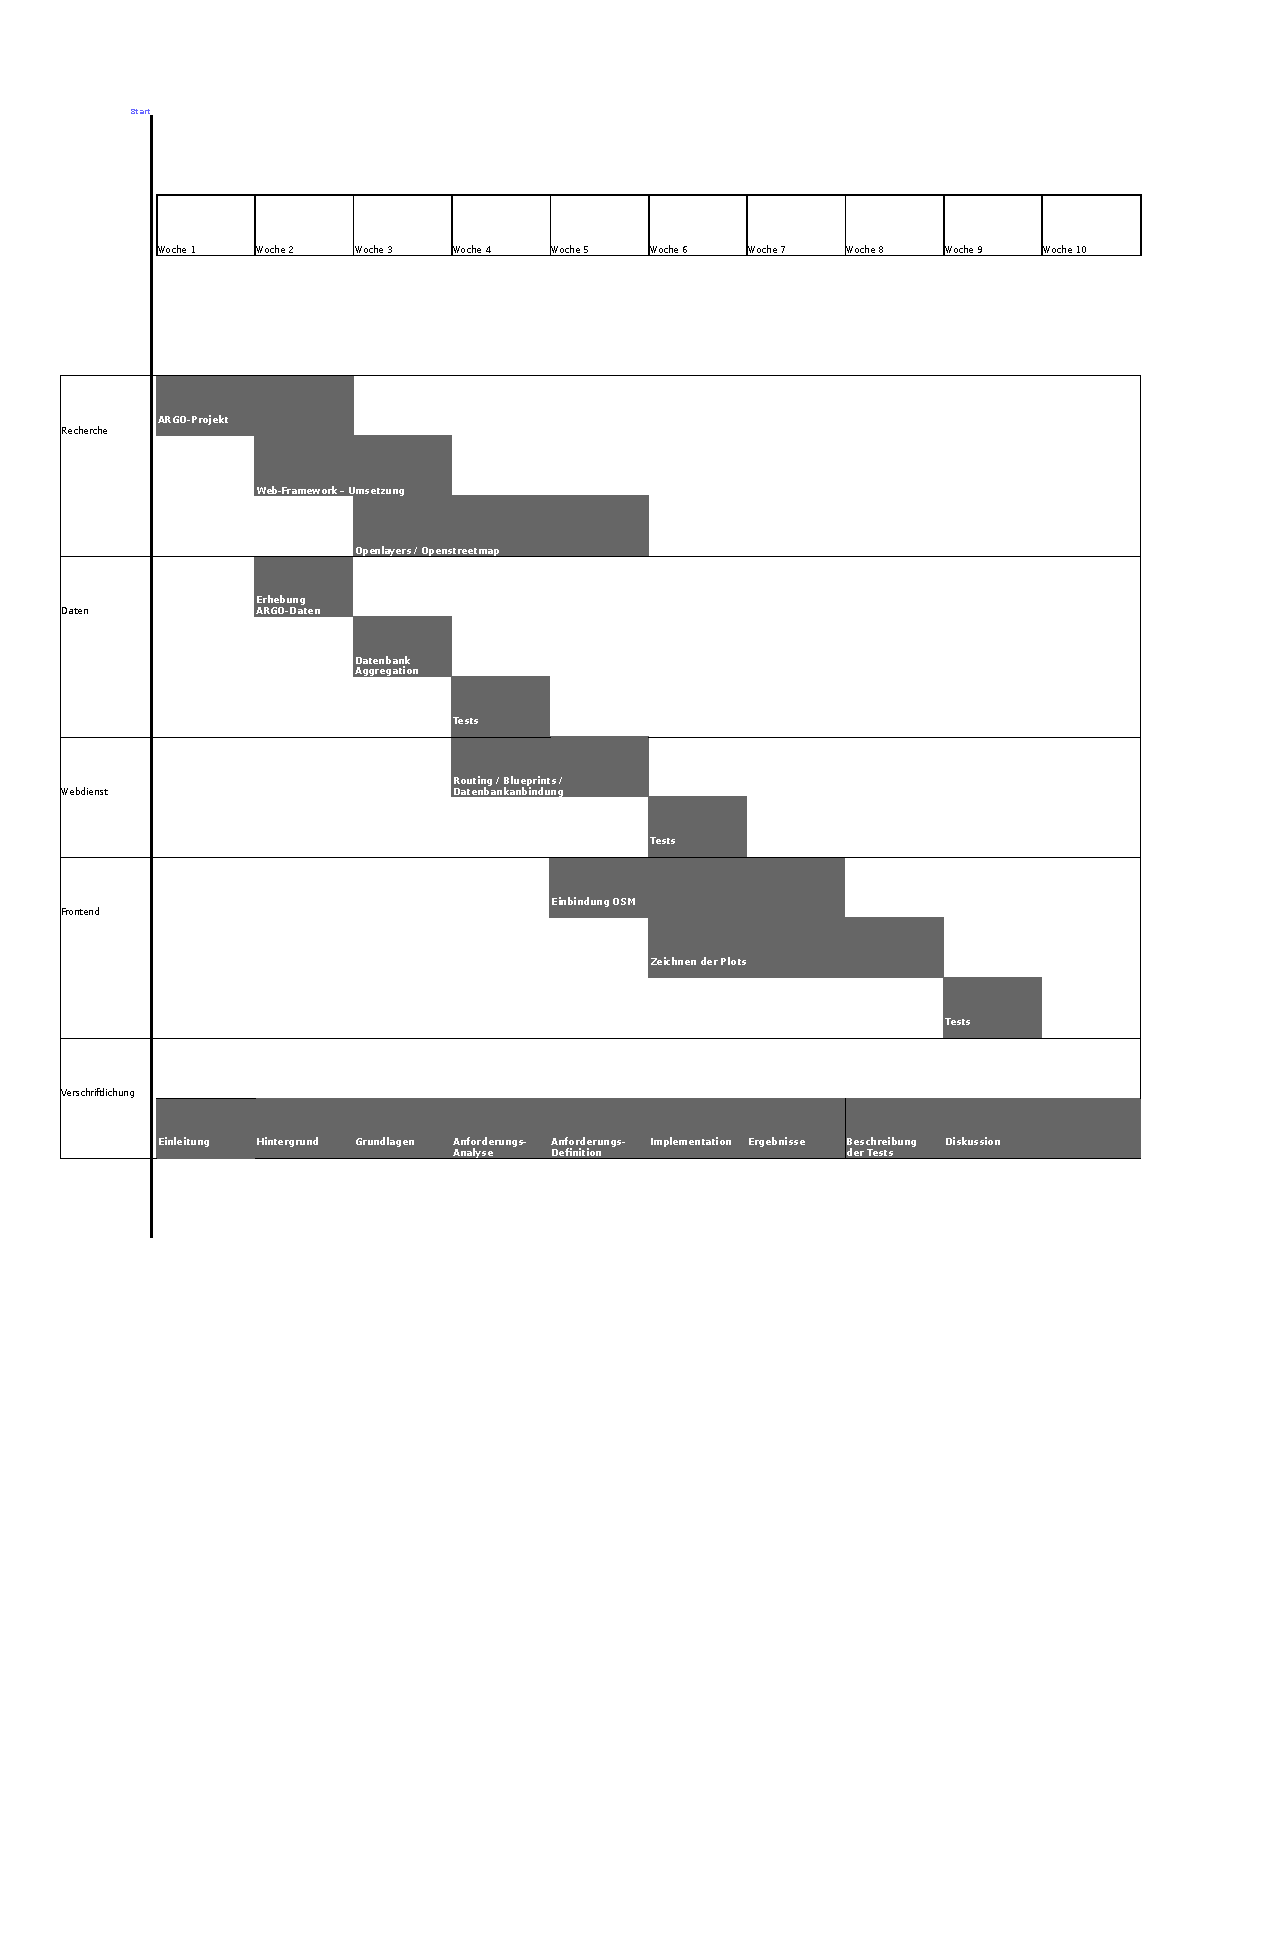
\includepdf[width=\paperwidth,clip,trim=0cm 10cm 0mm 1cm]{Zeitplan__.pdf}
\end{figure}




\bibliography{bib.bib}
\bibliographystyle{alpha}
\nocite{*}



%%%
%%%

%\include{Anhang}
\end{document} 
